\chapter{Kernel CN:\ Grammar}%
\label{chap:kernel-grammar}

\kl{CN} and \kl{Kernel} CN have different grammars. This is because \kl{CN} is
intended to be used by C programmers, whereas \kl{Kernel} CN is more for type
theorists, and also to be more convenient to work with as a formalism. The
primary differences are (a) \kl{CN} is implemented over (a version of)
\kl{Core}, whereas the \kl{kernel} is defined over a let-normalised version of
\kl{Core} (b) \kl{CN}'s grammar of types is close to the surface syntax and so
each construct serves many purposes whereas the \kl{kernel}'s grammar of types
is more traditional and each construct only serves one purpose.

In this chapter I will present the relevant parts of \kl{CN}'s syntax of
predicate definitions and assertions, and the \kl{kernel}'s syntax of types and
relevant terms, with a particular focus on explicit resource terms.

\section{CN Syntax}%

\begin{figure*}[tp]
    \centering
    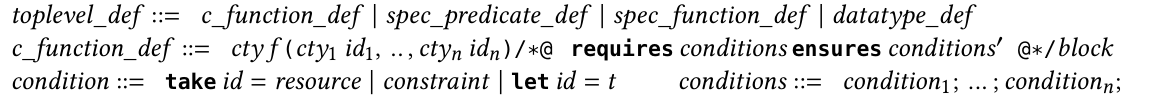
\includegraphics{figures/cn-grammar-1}
    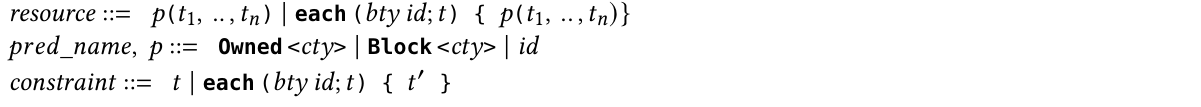
\includegraphics{figures/cn-grammar-2}
    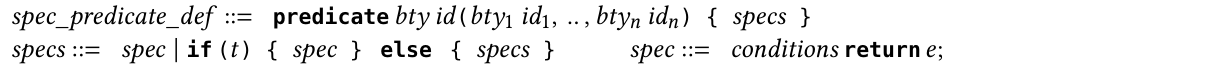
\includegraphics{figures/cn-grammar-3}
    \caption{Grammar of CN.}\label{fig:cn-grammar}
\end{figure*}

A file for \kl{CN} consists of series of top-level declarations of annotated C
functions, (separation logic) predicate definitions, (purely logical) function
definitions, and datatype declarations.\sidenote{Does the kernel formalism
support datatypes?} 

Function definitions for C introduce the identifiers for the arguments into the
scope of the pre- and postconditions, preceded by \cninline{requires} and
\cninline{ensures} respectively. Pre- and postconditions are a list of
`conditions', each followed by a semi-colon.
\begin{itemize}
    \item \cninline{take id = resource} is a \kl{monadic} bind, which bind
        the \emph{output} arguments of the resource to the identifier \cninline{id}.
    \item \cninline{constraint} is a boolean-valued expression.
    \item \cninline{let id = t} is simply an abbreviation for the expression \cninline{t} bound to \cninline{id}.
\end{itemize}

\kl{CN} constraints are either simple terms, or quantified
constraints.\sidenote{These must be manually instantiated by the user.}

\kl{CN} \kl{resource}s are simply a predicate \cninline{p(t1, .., tn)} % chktex 26 chktex 12 chktex 36
or an iterated predicate of the form
\cninline[breaklines]|each (<type> i; <guard>) { <pred>( array_shift(p i) ) }|. % chktex 36 chktex 37
Predicate names \cninline{p} are either \cninline{Owned<ct>}, representing ownership
of an initialised (read and write) location (a points-to $\mapsto{}$) indexed
by a C type, \cninline{Block<ct>} is similar but for an uninitialised (write only) location,
or a user-defined one.

\section{Desugaring CN types into kernel types}\label{sec:desugaring}

\subsection{Heap types}\label{subsec:heap-types}

\subsection{Resource Terms, Quantifier Inference}\label{subsec:resq-inf}

Explain \intro{bidirectional} (for quantifiers), linear resources, constraints.
Explicit witness to having permissions, which are linearly typed (just ingredients).
Explain enough rules \textemdash{} typing, operations, especially the weird heaps.
And of course, type safety statement and its proof.
Linear terms in a refinement type system.

(Dep ML, L3, F star, Jhala, ATS)

Different and unusual compared to Iris style \textemdash{} separation proofs outside the program.

Proof term in one sense, but also factors out operations for resource manipulation.

\subsection{Heaps}


\subsection{Type Safety}

\chapter{Kernel CN:\ Typing rules}%

\chapter{Kernel CN:\ Proof of soundness}%
\label{chap:kernel-soundness}

Weird heaps.
